%!TEX root = dgplvm.tex

\section{Introduction}
\label{cap:introduction}

\subsection{Why unsupervised learning}
\begin{frame}{Why unsupervised learning}
    Unsupervised learning is more subjective than supervised learning, as there is no simple goal for the analysis. But techniques for unsupervised learning are of growing importance in a number of fields:
    \begin{itemize}
        \pause
        \item visualize and draw trends of high dimensional problems,
        \pause
        \item subgroups of breast cancer patients grouped by their gene expression measurements,
        \pause
        \item groups of shoppers characterized by their browsing and purchase histories,
        \item movies grouped by the ratings assigned by movie viewers.
    \end{itemize}
\end{frame}

\begin{frame}{Examples of unsupervised learning}
    \begin{minipage}{.48\textwidth}
        \begin{figure}
            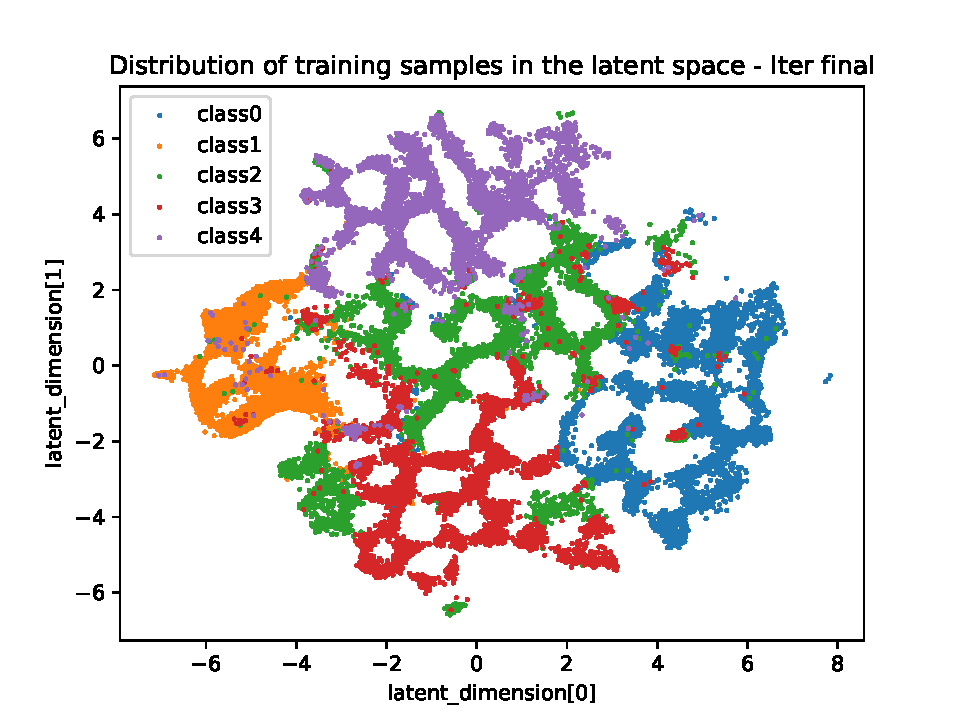
\includegraphics[width=\textwidth]{mnist_5classes_2dim.pdf}
            \caption{Feature projection of the \texttt{MNIST dataset} (5 digits)}
        \end{figure}
    \end{minipage}
    \begin{minipage}{.48\textwidth}
        \begin{figure}
            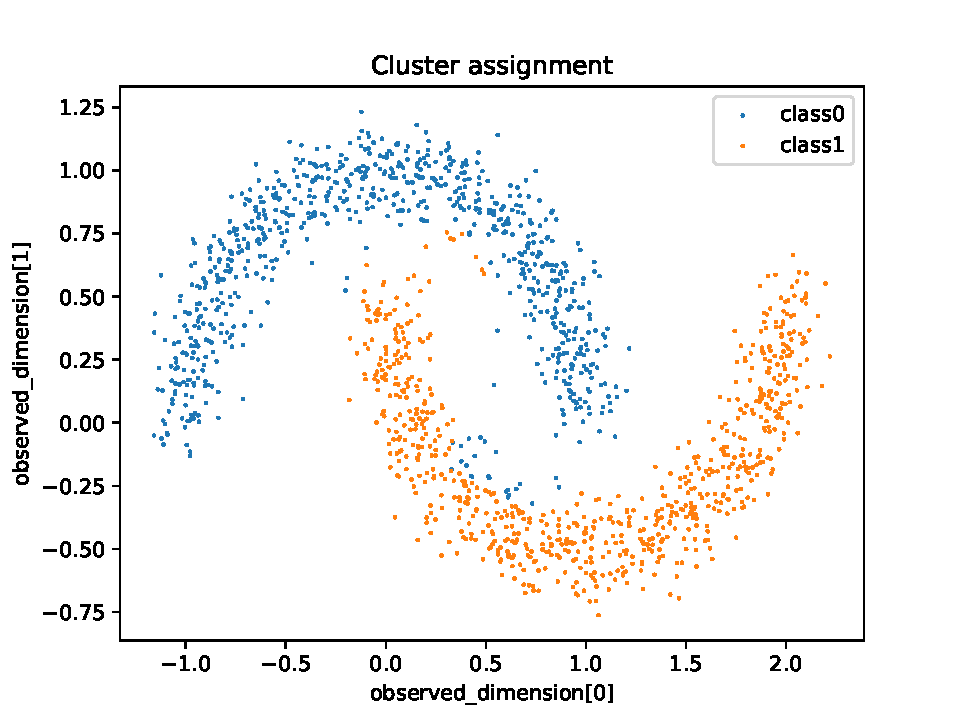
\includegraphics[width=\textwidth]{moons_assignment_cluster.pdf}
            \caption{Clustering assignment of the \texttt{sklearn} moon dataset}
        \end{figure}
    \end{minipage}
\end{frame}
